%!TEX root = hw1.tex
\problem{1}
\paragraph{a)} 
For the $O(n^2)$ solution we compute the intersection between one segment and the rest of the segments. Then we remove that segment and recursively compute the intersections between the rest of the segments.

\begin{algorithm}
	\caption{$O(n^2)$ solution for computing the number of intersections}
	\begin{algorithmic}
	  \Function{intersections}{$P[1..n]$ , $Q[1..n]$}
	  	\State $i \gets $ \Call{findIntersectionsWithSegment}{$P[1]$, $Q[1..n]$} \Comment{O(n)}
		\State \Call{removePointAt}{{$i+1$, $Q[1..n]$}} \Comment{O(n)}
	
		\Return $i + \Call{intersections}{$P[2..n]$, $Q[1..n-1]$}$
	  \EndFunction
	
	  \Function{findIntersectionsWithSegment}{$p$ , $Q[1..n]$}
		\State $i \gets 0$
		\While{$Q[i] < p$}
			\State $i \gets i + 1$
		\EndWhile
	
		\Return $i$
	  \EndFunction
	
	  \Function{removePoint}{$i$, $Q[1..n]$}
		\For{$j \gets i, n-1$}
			\State $Q[i] \gets Q[i + 1]$
		\EndFor
	  \EndFunction
	\end{algorithmic}
\end{algorithm}

\paragraph{Runtime analysis}
Functions $findIntersectionWithSegment$ and $removePoint$ have a runtime of $O(n)$ since in the worst case scenario they traverse over all all the points. The runtime of function $intersections$ is analyzed below: \\

$I(n) =$ worst case runtime of function $intersections$

$I(n) = I(n - 1) + 2 * O(n)$

\begin{figure}[H]
    \centering
    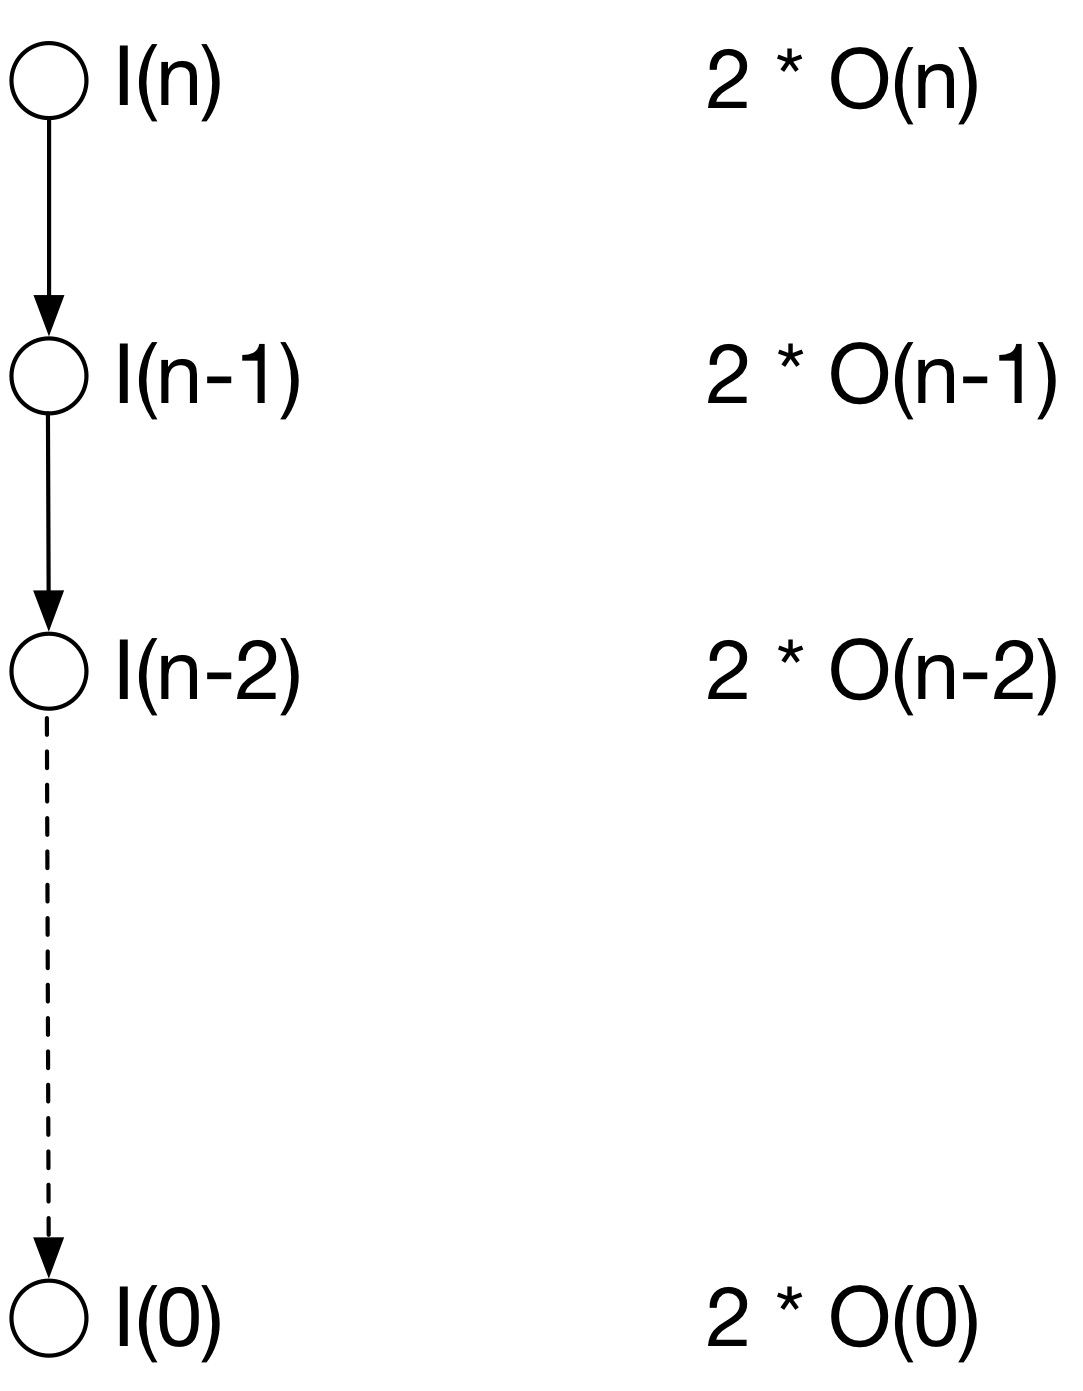
\includegraphics[scale=0.4]{1a)}
\end{figure}

$I(n) = \sum_{i=0}^{n} 2 * O(i) = 2 * \sum_{i=0}^{n} O(i) \Rightarrow  2 * O(n^2) \Rightarrow  O(2 * n^2) \Rightarrow O(n^2)$


\paragraph{b)} For the $O(n*log(n))$ solution we sort the P array of points and perform the same swaps within Q that are required to sort P.
This operation preserves the number of intersections from the initial arrays.
Figure \ref{fig:pointSwap} shows that, in the base case when there are either two parallel segments or two intersecting segments, the number of intersections is preserved when the order of the points is swapped.

\begin{figure}
    \centering
    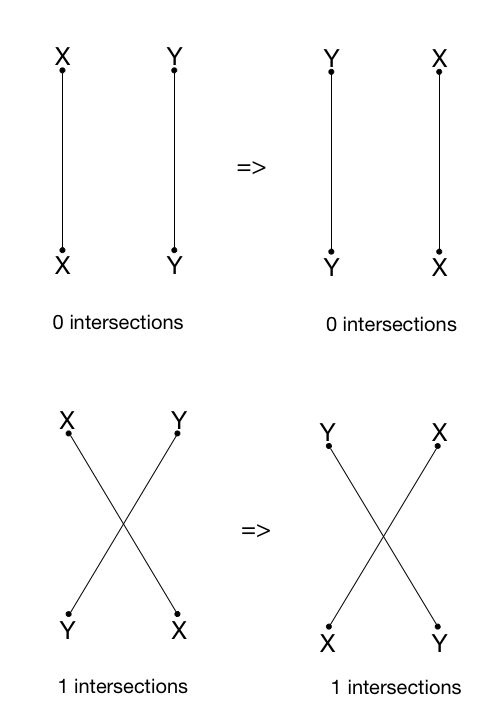
\includegraphics[scale=0.35]{1b-intersections}
    \caption{The number of intersections is preserved when swapping points}
    \label{fig:pointSwap}
\end{figure}

Having P sorted, we can now compute the number of intersections by looking only into the Q array. We achieve this via a modified merge sort, the number of intersection for Q being: \\

$intersections(Q[1..n]) = intersections(Q[1 .. \lfloor n/2 \rfloor]) + intersections(Q[\lceil n/2 \rceil .. n]) + merge(Q[1 .. \lfloor n/2 \rfloor], Q[\lceil n/2 \rceil .. n])$ \\

The $merge$ function, just like in the traditional merge sort, merges the two sorted arrays into one sorted array. 
Additionally, it computes the number of intersections between the two arrays: whenever a number from the rightmost array is copied into the merged array, it generates as many intersections as numbers are left in the leftmost array.

Figure \ref{fig:pointInd} illustrates how the merging is done, assuming recursion solved the smaller cases. 
The figure shows the case of an $n$ array of points where $n-1$ points have been sorted.
One segment, $j$, such that $i \leq j < k$ remains unsorted.
In order to put $j$ into its place we need to swap it over the interval $[k .. n]$ of points, thus generating $m = n - k + 1$ intersections.
Similarly, if there are more unsorted points, each one is moved into its place while generating as many intersections as many points it crosses.

\begin{figure}[H]
    \centering
    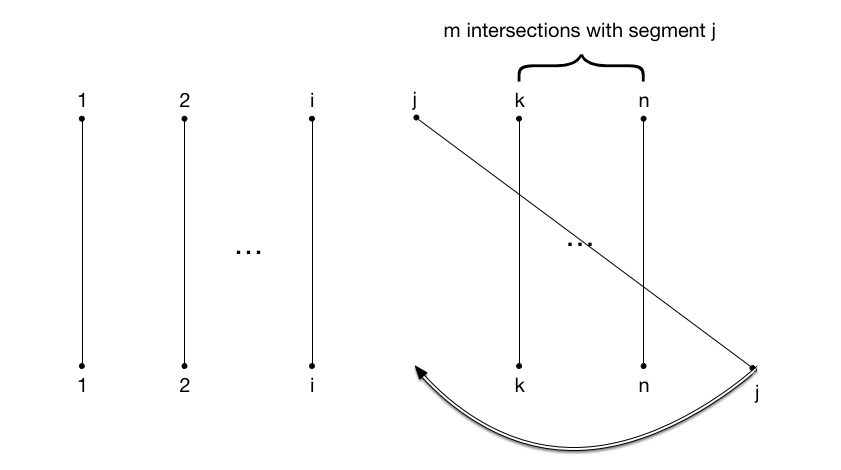
\includegraphics[scale=0.35]{1b-intersections-ind}
    \caption{Computing the number of intersections in an $n$ array of points, where $n-1$ points are already sorted}
    \label{fig:pointInd}
\end{figure}

\begin{algorithm} [H]
	\caption{$O(n * log(n))$ solution for computing the number of intersections}
	
	\begin{algorithmic}
	  \Function{intersections}{$P[1..n]$ , $Q[1..n]$}
	  	\State \Call{sortInParallel}{$P[1..n]$,$Q[1..n]$} \Comment{$O(n*log(n))$}
		
		\Return \Call{mergeIntersections}{$Q[1..n]$} \Comment{$O(n*log(n))$}
	  \EndFunction
	  
	  \Function{sortInParallel}{{$P[1..n]$ , $Q[1..n]$}}
	  	\LineComment{Sort P using an $O(n * log(n))$ sorting algorithm. $Q[i]$ and $Q[j]$ are swapped whenever $P[i]$ and $P[j]$ are swapped. See Figure \ref{fig:pointSwap}.}
	  \EndFunction
	  
	  \Function{mergeIntersections}{$Q[1..n]$}
		\If {$n = 1$}
		
			\Return 0
		\EndIf
	  
	  	\State $m \gets \lfloor n/2 \rfloor$
		\State $i1 \gets \Call{mergeIntersections}{Q[1 .. m}$	
		\State $i2 \gets \Call{mergeIntersections}{Q[m + 1 .. n}$
		\State $i3 \gets \Call{merge}{Q[1 .. n], m}$ \Comment{$O(n)$}
	 
	 	\Return $i1 + i2 + i3$
	  \EndFunction
	  
	  \Function{merge}{$Q[1..n], m$}
	  	\State $i \gets 1$
	  	\State $j \gets m + 1$
		\State $k \gets 1$
	  	\State $intersections \gets 0$
		
		\While{$i < m \wedge j < n$}
			\If{$Q[i] < Q[j]$}
				\State $B[k] \gets Q[i]$
				\State $i \gets i + 1$ 
				\State $k \gets k + 1$
			\Else
				\State $B[k] \gets Q[j]$
				\State $intersections = intersections + (m - i) + 1$
				\State $j \gets j + 1$ 
				\State $k \gets k + 1$
			\EndIf
		
			\For{$k \gets 1, n$}
				\State $Q[k] \gets B[k]$
			\EndFor
			
		\EndWhile
		
	\Return $intersections$
	\EndFunction
	  
	\end{algorithmic}
\end{algorithm}

\paragraph{Runtime analysis}
	  
Function $intersections$ has a runtime of $2*O(n* log(n)) = O(n* log(n))$
Function $sortInParallel$ is based on an $O(n* log(n))$ sorting algorithm such as merge sort.
Function $merge$ has a runtime of $2*O(n) = O(n)$ since it contains two loops that iterate over all the elements of the parameter.
The runtime for $mergeIntersections$ is analyzed below: \\

$I(n) =$ worst case runtime of function $mergeIntersections$

$I(n) = 2 * I(n/2) + O(n)$

\begin{figure}[H]
    \centering
    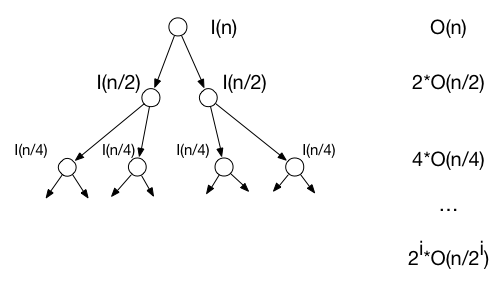
\includegraphics[scale=0.4]{1b-runtime}
\end{figure}

$I(n) = \sum_{i=1}^{L} 2^i * O(n/2^i) = \sum_{i=1}^{L} O(n) \Rightarrow L * O(n)$

L is the height of the tree, $log(n)$

$I(n) = log(n) * O(n) \Rightarrow O(n*log(n))$

